\section{Introduction}
\subsection{Overview of Flyback Converters}
A flyback converter is a kind of isolated switched-mode power supply (SMPS) that isolates its input and output stages electrically by using a transformer. Modern power electronics are built on this isolation, which guarantees safety and adherence to legal requirements. The ability of flyback converters to offer several regulated output voltages, their affordability, and their small size have made them well-known and solidified their place in a variety of applications, from industrial systems to consumer electronics. In applications where efficiency and space are crucial, such as LED drivers, phone chargers, and television auxiliary power sources, they are essential.\\[0.3cm]
The significance of flyback converters has increased in today's technologically advanced world due to the rising need for dependable, lightweight, and energy-efficient power solutions. Because of their straightforward design and ability to function in both continuous conduction mode (CCM) and discontinuous mode (DCM), engineers may customize them to meet a range of power needs.
\begin{multicols}{2}  % Start two-column layout
    % First column: image 1
    \noindent
    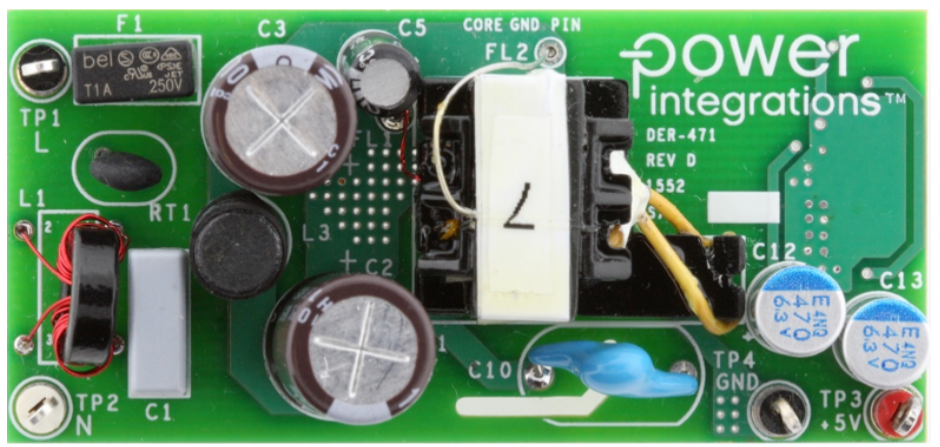
\includegraphics[width=1\linewidth]{Pictures/pics/1.png}
    \captionof{figure}{\textcolor{blue}{\textit{\footnotesize15-W Isolated Flyback Converter}}}
    \hfill
    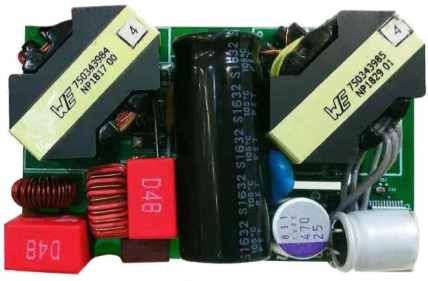
\includegraphics[width=0.8\linewidth]{Pictures/pics/2.png}
    \captionof{figure}{\textcolor{blue}{\textit{\footnotesize 100-W AC/DC adapter}}}
\end{multicols}
\subsection{Purpose of the Report}
% \noindent % To make sure the text starts immediately after the multicolumn environment ends
\noindent The purpose of this report is to provide a comprehensive analysis of flyback converters, focusing on their working principle, key design considerations, and practical applications. By exploring these aspects, the report aims to highlight the technical nuances that make flyback converters indispensable in modern electronics while addressing challenges such as leakage inductance, switching losses, and electromagnetic interference (EMI).

% % Now switching to single-column layout for the next figure and caption
\begin{figure}[h!]
    \centering
    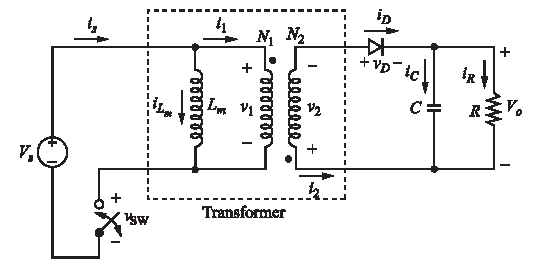
\includegraphics[width=0.6\linewidth]{Pictures/pics/6.pdf}
    \caption{\textcolor{blue}{\textit{\footnotesize Equivalent circuit using a transformer model that includes the magnetizing inductance}}}
\end{figure}